\subsection{Modes, Sizes and Tolerances}
\label{app:verification-modes}

A block encoding $(U,\alpha)$ of an operator $X$ is exact when $\alpha\,\Pi_{\mathrm{out}}U\Pi_{\mathrm{in}}=X$, the projectors fixing the ancilla at zero. Every mode of \Cref{tab:verification-modes} compares that block, or its action on vectors, with a target built from the problem by the operator library and the residual's assembly, never from the compiler that produced the circuit; a target rebuilt from the circuit's own parts would check the compiler against itself. The pipeline's usual target is the stacked reflection's block $2H/\alpha_R^2-I$ with $H$ formed from the assembled residual; the atoms (the derivative, a lift, a feature-map row) are compared with their operators in the same way.

\paragraph{Exact.} The whole block is reconstructed, one statevector evolution per input basis vector, and its largest entrywise error $\|E\|_{\max}$ is compared with $10^{-10}\|X\|_2$. An $r\times c$ block within that tolerance entry by entry has $\|E\|_2\le\sqrt{rc}\,\|E\|_{\max}$, so the mode certifies the circuit completely at that size. Its cost is $c$ evolutions of $2^q$ amplitudes.

\paragraph{Probe.} The circuit is applied to $4$ structured vectors and $16$ Haar-random ones, each one evolution at any size, and compared with a sparse product of the target, which is never formed densely; a probe $v$ passes when $\|Ev\|\le10^{-9}\max(1,\|Xv\|)$, the random probes seeded by the run.

\begin{proposition}[What random probes see]
\label{prop:haar-probes}
For $\psi$ Haar-distributed on dimension $D$,
\begin{equation*}
    \mathbb{E}\,\|E\psi\|^2=\frac{\|E\|_F^2}{D}.
\end{equation*}
If the error lies in one column, $E=\delta\,w\,e_j^\dagger$ with $\|w\|=1$, then $\|E\psi\|=\delta|\psi_j|$ and $D|\psi_j|^2$ has mean one.
\end{proposition}
\begin{proof}
$\mathbb{E}\,\psi\psi^\dagger=I/D$, so $\mathbb{E}\|E\psi\|^2=\operatorname{tr}(E^\dagger E)/D$; for the column error $\|E\psi\|^2=\delta^2|\psi_j|^2$.
\end{proof}

Random probes therefore estimate the root-mean-square error $\|E\|_F/\sqrt D$, and an error of size $\delta$ confined to one column is seen at about $\delta/\sqrt D$: caught with certainty only when $\delta\gtrsim10^{-9}\sqrt D$. The probe mode is evidence of correctness, not a proof of it. Unlike the exact mode, whose cost grows with the number of input columns, it costs twenty evolutions at any size, so it runs on every circuit of at most 24 qubits that the exact mode does not cover.

\paragraph{IR.} The compiled terms of a descriptor residual, a coupling or a lift are summed back into a sparse matrix and compared with the operator assembled from the problem, entry by entry relative to its norm, at tolerance $10^{-10}$, at any size and with no simulation (\Cref{app:term-ir}). The two sides are independent constructions, so the comparison is not a tautology. What it leaves open is the step from terms to gates, which the exact and probe modes check where a circuit can be simulated. Together they chain: the assembled operator equals the terms at every $n$, and the terms equal the circuit at every simulable size. The compiler is structural, one atom per term, so the circuit at a larger size is the same construction, but it is not independently verified there.

\paragraph{Approximation.} Wu et al.'s approximate encoding of $\G$ (\Cref{app:published-build}) is compared with $\G$ and its entrywise error reported beside the bound of \Cref{prop:epsilon-G}; the mode never fails, since the encoding is approximate by design and enters resource estimates only.

Circuits wider than the probe ceiling are construction-only records: their subnormalisation, register split and gate counts are recorded, with no verdict.

The four structured inputs of the probe mode are placed where a defect confined to one column arises, because a random input sees such a defect only at about $\delta/\sqrt D$ (\Cref{prop:haar-probes}), while the basis vector that selects its column sees it at full strength. The first basis vector is the $T_0$ mode and the start of every chain of shifts, and the last is where a truncated shift must not wrap round to the start of the register. The middle one, index $D/2$, sets only the most significant qubit, so it sits on the edge between the two halves of a register and between the blocks of a padded state, where block offsets and axis orders go wrong; the uniform vector tests the sum of all columns at once. A defect in a column that none of them selects is left to the random probes. Every atom is also verified alone before it is composed: the structured factorisation of $\G$ (\Cref{app:structured}), the lifts and folds, the feature-map rows, each band of the descriptor (\Cref{app:term-ir}) and the matchings of a coupling, each exactly at small $n$ and by probe or \gls{ir} beyond; the banded factorisation $\Bt\G=\Dt$ holds to rounding for $n=1$ to $10$. The composed reflection is then verified whole, so that correct atoms cannot hide an error made in composing them, such as a wrong block offset or a mis-ordered register.

\subsection{The Classical Reference: Eigensolver Against SVD}
\label{app:eigh-vs-svd}

The reference is the smallest right singular vector of $R$, computed by a backward-stable \gls{svd} (LAPACK's divide-and-conquer driver, with the QR-based driver where it fails to converge), in double precision only; $H$ is never formed.

\begin{proposition}[The two bounds]
\label{prop:wedin}
A backward-stable \gls{svd} returns the exact singular vectors of $R+\delta R$ with $\|\delta R\|_2\le c\,\epsilon_{\mathrm{mach}}\sigma_{\max}$, and the computed ground state makes with the exact one an angle with
\begin{equation}
    \sin\vartheta_{\mathrm{SVD}}\le\frac{\|\delta R\|_2}{\sigma_1-\hat\sigma_0}\approx\frac{c\,\epsilon_{\mathrm{mach}}\sigma_{\max}}{\sigma_1-\sigma_0},
    \label{eq:wedin}
\end{equation}
$\hat\sigma_0$ the perturbed value. A backward-stable symmetric eigensolver applied to the formed $H$ returns the eigenvectors of $H+\delta H$ with $\|\delta H\|_2\approx c\,\epsilon_{\mathrm{mach}}\sigma_{\max}^2$, and
\begin{equation*}
    \sin\vartheta_{\mathrm{eig}}\lesssim\frac{c\,\epsilon_{\mathrm{mach}}\sigma_{\max}^2}{\sigma_1^2-\sigma_0^2}.
\end{equation*}
\end{proposition}
\begin{proof}
The first is Wedin's $\sin\Theta$ theorem for singular subspaces \cite{wedin1972perturbation} applied to the perturbation $\delta R$; the second is the Davis--Kahan theorem \cite{daviskahan1970rotation} applied to $\delta H$, with the gap $\lambda_1-\lambda_0=\sigma_1^2-\sigma_0^2$.
\end{proof}

The ratio of the two is $\sigma_{\max}/(\sigma_1+\sigma_0)$, the residual's condition number on the complement of its near-kernel: the eigensolver loses that factor. When $\sigma_0\ll\sigma_1$ the SVD's bound is about $\epsilon_{\mathrm{mach}}\sqrt{\|H\|/\Delta}$, the square root of the eigensolver's. Both require $\sigma_0$ to be isolated, the trusted-kernel condition of \Cref{app:trust-threshold}. On the standard form the eigensolver's bound grows with $n$ by the factor that $\sigma_{\max}/\sigma_1$ grows, $2^{2k}$ per qubit at order $k$, until it saturates, and Wedin's, smaller by that factor, stays below one; on R2a the eigensolver's angle reaches order one by $n=8$, where the SVD's is still small (\Cref{tab:eigh-vs-svd}). The bounds are what a backward-stable algorithm can promise: on the standard form the smallest singular value is returned at the floor $\epsilon_{\mathrm{mach}}\sigma_{\max}$ rather than at its true, smaller value, which is why the kernel is detected by a ratio against that floor. A single-precision residual has $\epsilon_{32}\sigma_{\max}/(\sigma_1-\sigma_0)>10^{-3}$ on R2a from $n=5$, and is refused.

\begin{table}[htbp]
    \centering
    \caption[Accuracy of the classical reference: eigensolver against SVD]{\textbf{The eigensolver loses the residual's condition number; the SVD does not.} Sine of the angle between the classical reference and the state of the exact coefficients on R2a ($f''+4f'+4f=0$): the standard form by a symmetric eigensolver on $R_{\mathrm{std}}^{\top}R_{\mathrm{std}}$ and by \gls{svd} of $R_{\mathrm{std}}$, and the descriptor by \gls{svd}, on its physical columns. At $n=2$ and $3$ the truncation dominates both routes; from $n=4$ the angle is the solver's. Classical computation.}
    \label{tab:eigh-vs-svd}
    \small
    \begin{tabular}{@{}r l l l@{}}
        \toprule
        $n$ & Standard, eigensolver & Standard, SVD & Descriptor \\
        \midrule
        2 & $\res[2,sci]{reference/R2a/standard/n2}{eigh_sine}$ & $\res[2,sci]{reference/R2a/standard/n2}{svd_sine}$ & $\res[2,sci]{reference/R2a/descriptor/n2}{svd_sine}$ \\
        3 & $\res[2,sci]{reference/R2a/standard/n3}{eigh_sine}$ & $\res[2,sci]{reference/R2a/standard/n3}{svd_sine}$ & $\res[2,sci]{reference/R2a/descriptor/n3}{svd_sine}$ \\
        4 & $\res[2,sci]{reference/R2a/standard/n4}{eigh_sine}$ & $\res[2,sci]{reference/R2a/standard/n4}{svd_sine}$ & $\res[2,sci]{reference/R2a/descriptor/n4}{svd_sine}$ \\
        5 & $\res[2,sci]{reference/R2a/standard/n5}{eigh_sine}$ & $\res[2,sci]{reference/R2a/standard/n5}{svd_sine}$ & $\res[2,sci]{reference/R2a/descriptor/n5}{svd_sine}$ \\
        6 & $\res[2,sci]{reference/R2a/standard/n6}{eigh_sine}$ & $\res[2,sci]{reference/R2a/standard/n6}{svd_sine}$ & $\res[2,sci]{reference/R2a/descriptor/n6}{svd_sine}$ \\
        7 & $\res[2,sci]{reference/R2a/standard/n7}{eigh_sine}$ & $\res[2,sci]{reference/R2a/standard/n7}{svd_sine}$ & $\res[2,sci]{reference/R2a/descriptor/n7}{svd_sine}$ \\
        8 & $\res[2,sci]{reference/R2a/standard/n8}{eigh_sine}$ & $\res[2,sci]{reference/R2a/standard/n8}{svd_sine}$ & $\res[2,sci]{reference/R2a/descriptor/n8}{svd_sine}$ \\
        \bottomrule
    \end{tabular}
\end{table}

\subsection{The Iterative Reference}
\label{app:iterative-reference}

Beyond $8{,}192$ physical columns the dense \gls{svd} takes too long and too much memory, and the smallest singular triplets are found iteratively. Lanczos iteration finds the largest eigenvalues of a symmetric operator, and the smallest singular values of $R$ are the largest eigenvalues of $(R^\dagger R+\mu I)^{-1}$, which is applied without forming $R^\dagger R$.

\begin{proposition}[The augmented system]
The solution of $\bigl(\begin{smallmatrix}I&R\\R^\dagger&-\mu I\end{smallmatrix}\bigr)\bigl(\begin{smallmatrix}r\\x\end{smallmatrix}\bigr)=\bigl(\begin{smallmatrix}0\\c\end{smallmatrix}\bigr)$ has $x=-(R^\dagger R+\mu I)^{-1}c$.
\end{proposition}
\begin{proof}
The first row gives $r=-Rx$; substituting, $-R^\dagger Rx-\mu x=c$.
\end{proof}

One sparse LU factorisation of the augmented matrix serves every Lanczos step. It does not fill as the normal matrix does: a dense constraint row of $R$, with $N$ entries, appears once in $R$ and once in $R^\dagger$, where it would put a dense $N\times N$ block into $R^\dagger R$.

\paragraph{Upper bounds and the a posteriori estimate.} For $V$ with orthonormal columns, the $j$-th smallest singular value of $RV$ is at least the $j$-th smallest of $R$ (Cauchy interlacing), so the computed $\tilde\sigma_0$ and $\tilde\sigma_1$ never fall below the true ones. For the returned $v$, with $r=\|Rv\|\ge\sigma_0$, the infidelity against the true ground state $v_\star$ satisfies $1-|\braket{v|v_\star}|^2\le(r^2-\sigma_0^2)/(\sigma_1^2-\sigma_0^2)\le r^2/\sigma_1^2$, and the reported bound is $r^2/(\tilde\sigma_1^2-r^2)$, which is at least $r^2/\sigma_1^2$ when no singular value below $\tilde\sigma_1$ is missed. It is therefore an estimate, exact to rounding once the iteration has converged and nothing below $\tilde\sigma_1$ is missing; it floors at about $(\sigma_0/\sigma_1)^2$ where $R$ has no kernel, and is sharp where it has one.

\paragraph{The start vector.} Both Lanczos runs start from a Gaussian vector of fixed seed: deterministic, answer-independent and with a component on every singular vector. A uniform start would not do: if a permutation $P$ of the columns commutes with $R^\dagger R$ and $Pu=u$, every Krylov vector is $P$-fixed, so the iteration never meets a singular vector of another symmetry sector. On the Taylor--Green vortex, whose residual has such a symmetry, a uniform start misses most of the lowest singular values.

\paragraph{Checks.} The iterative reference reaches residuals of \res{build/R10d-M48/descriptor/n4/carleman=3}{dimension} columns, on the Navier--Stokes lifts. Where both run, it reproduces the dense one's ground state to the dense one's own error. Past the standard form's moderate $n$, where the dense \gls{svd}'s backward error $\epsilon_{\mathrm{mach}}\sigma_{\max}$ is no longer small against $\sigma_1$, the iterative reference is the more accurate: on R2a from $n=8$ to $10$ its $\sigma_1$ varies by $\res[1,sci]{iterative/R2a/standard/drift}{iterative_spread}$ relative, where the dense value varies by $\res[1,sci]{iterative/R2a/standard/drift}{dense_spread}$, and on the descriptor there the two agree to $\res[2]{iterative/R2a/descriptor/range}{high}\,\epsilon_{\mathrm{mach}}\sigma_{\max}$.

\subsection{The Trust Threshold}
\label{app:trust-threshold}

The ascending singular values are floored at $10^{-300}$, so that an exact zero gives a finite ratio, and the ratios $\sigma_k/\sigma_{k-1}$ are formed for $k=1,\dots,16$. The kernel's dimension is the $k$ of the largest ratio, the \emph{gap ratio} is that ratio, and the reference is trusted when the dimension is one and the gap ratio at least $20$. An exact kernel of dimension $k$ is found because its computed values are at most $c\,\epsilon_{\mathrm{mach}}\sigma_{\max}$ by Weyl's inequality, so its ratio exceeds $20$ whenever $\sigma_k/\sigma_{\max}$ exceeds about $4\times10^{-15}$; beyond that the floor is the gap's own size and nothing in the computed spectrum separates them. For a near-kernel, if the truncated solution $\hat b$ nearly minimises the residual, $\|R\hat b\|\approx\sigma_0$, its angle to the ground state is at most about $\sigma_0/\sigma_1$: a gap ratio of $20$ puts the ground state within $0.05$ of it in sine.

\paragraph{Why $20$.} A spectrum with no kernel still has ratios, and the detector reports the largest as a kernel's. The threshold must exceed the largest ordinary spacing in the benchmark problems' singular spectra, so that a ratio above it cannot come from spacing alone. Over the classical builds of R1 to R8 the largest such spacing is the stiff R2c's structural $\sigma_2/\sigma_1$, just under $20$, with the median far below; the only larger ratios are those of three of the reproduction's panels (\Cref{app:reproduction}), whose second near-kernel is not a spacing. The value is empirical, a property of these spectra and not a theorem.

\paragraph{What it does not decide.} A kernel of dimension above one is never trusted; the doubled space's is the example (\Cref{sec:doubled-space}). A second near-kernel higher up, with a larger ratio, moves the reported dimension above one and is untrusted, which is conservative. A one-dimensional kernel with a modest gap ratio, an under-resolved problem found by luck, is not trusted. An iterative reference counts among its smallest seventeen values with the Ritz upper bounds above, and can report a ratio too small by their overestimate. Trust means that a kernel is detected, not that the field has converged; the convergence in $n$ is measured separately.

\subsection{The Circuit-Simulation Memory and Time Model}
\label{app:t1-model}

A circuit simulation applies the \gls{gqsp} circuit one controlled walk at a time on a statevector simulator \cite{qiskit2024}, with gate fusion off, on the walk's qubits and the signal, $q=q_W+1$; it holds a statevector, never an operator, so its memory grows as $2^q$ and not $4^q$ (\Cref{app:controlled-walk}).

\paragraph{Memory.} A statevector of $q$ qubits is $S=16\cdot2^q$ bytes of complex double-precision amplitudes, and a dense $k$-qubit gate matrix $16\cdot4^k$ bytes, totalling $G$ over a step's dense gates. The peak resident memory is estimated as
\begin{equation*}
    M_{\mathrm{peak}}=M_0+8S+4G,
\end{equation*}
with $M_0$ the interpreter and libraries, eight statevector-sized buffers at the simulation's peak and four copies of each gate matrix. The multipliers are measured, not derived, from $20$ to $24$ qubits, and the model's peak is within $0.85$ to $1.05$ of the memory resident in a fresh process at $22$ qubits. The statevector term alone is $2^{q-23}$\,GiB: $8$\,GiB at $26$ qubits and $128$\,GiB at $30$. Memory is the hard limit of circuit simulation; time is the soft one.

\paragraph{Time.} Once the memory fits, one step is simulated untimed to warm the caches, then five times, and the median is $t_{\mathrm{step}}$; a single cold step on a shared node can read many times its steady cost, and the median of warm steps does not move for one slow outlier. The run's estimate is $(\text{candidates})\cdot(d+1)\cdot t_{\mathrm{step}}$, $d+1$ steps for the degree and the opening rotation and one simulation per initial-state candidate. Which resolutions circuit simulation reaches is therefore a joint statement of $q$ and $d$: the degree is set by the spectrum, and one more qubit roughly doubles both the memory and the step's time.

\paragraph{Refusal.} The budget is the job's allocation of memory and time. The estimate is logged against it whatever the verdict, and a run that exceeds either is refused and recorded as beyond the simulation budget, with the estimate and the resource estimate's numbers beside it; if the memory does not fit, the step is never timed.

\subsection{Acceptance and the Error Budget}
\label{app:error-budget}

\begin{table}[htbp]
    \centering
    \caption[Acceptance criteria for a state preparation]{\textbf{Every preparation is judged at five levels, each against a bar it can be measured to.} Applied to every preparation whose reference is trusted; a run that fails a bar is reported as a finding, never re-judged. $\psi$, $\psi_{\mathrm{ref}}$, prepared and reference states; $\varepsilon$, target suppression; $p_G$, post-selection success probability; $d$, filter degree; $\varepsilon_{\mathrm{disc}}$, discretisation error; $B(d_{\mathrm{total}})$, the error budget. The state bar's a priori bound follows from the spectral edge, $\gamma$ and the filter (\Cref{prop:minimax-guarantee}); the circuit bar is judged before normalising, which divides rounding by $\sqrt{p_G}$, and on normalised states only where $p_G\ge10^{-12}$ (\Cref{lem:normalising}).}
    \label{tab:acceptance}
    \small
    \begin{tabular}{@{}l p{0.44\linewidth} p{0.34\linewidth}@{}}
        \toprule
        Level & Measured & Bar \\
        \midrule
        State & infidelity $1-|\braket{\psi_{\mathrm{ref}}|\psi}|^2$ in the form's own space & $\le\varepsilon=10^{-6}$, and $\le10\times$ its a priori bound \\
        Circuit & circuit simulation against exact emulation from a unit input, before normalising & $\le10^{-10}$ \\
        Probability & the two tiers' $p_G$ & relative $\le10^{-8}$ \\
        Phases & realised \gls{gqsp} polynomial against its target, on $4(d+1)$ points of the unit circle & $\le10^{-12}$ \\
        Field & decoded field against the reference solution, $L^\infty$ & $\le\varepsilon_{\mathrm{disc}}+B(d_{\mathrm{total}})$, \Cref{eq:error-budget} \\
        \bottomrule
    \end{tabular}
\end{table}

\begin{lemma}[Normalising amplifies differences]
\label{lem:normalising}
For non-zero vectors $x$ and $y$, $\bigl\|x/\|x\|-y/\|y\|\bigr\|\le2\|x-y\|/\|x\|$, and $\bigl|\|x\|^2-\|y\|^2\bigr|\le\|x-y\|(\|x\|+\|y\|)$.
\end{lemma}
\begin{proof}
$\bigl\|x/\|x\|-y/\|y\|\bigr\|\le\|x-y\|/\|x\|+\|y\|\,\bigl|1/\|x\|-1/\|y\|\bigr|=(\|x-y\|+|\|y\|-\|x\||)/\|x\|$, and the reverse triangle inequality bounds the second term by $\|x-y\|$. The second inequality factorises a difference of squares.
\end{proof}

The circuit's output has norm $\sqrt{p_G}$, so a rounding error of about $10^{-16}$ in the unnormalised output becomes about $10^{-16}/\sqrt{p_G}$ in the normalised state; at $p_G=10^{-12}$ that is the bar of $10^{-10}$. The circuit and its emulation are therefore compared before normalising, from a unit input, and the normalised states only where $p_G\ge10^{-12}$; below it the comparison would measure rounding, not the circuit. The probability bar follows from the circuit bar by the lemma's second part only for $p_G\gtrsim4\times10^{-4}$, and is a separate measurement below. A run that fails a bar is reported as a finding, with its degree and the growth of the difference, and never re-judged against an adjusted bar.

\paragraph{The state metric.} For unit vectors the distance between states, $d(a,b)=\min_\phi\|a-e^{\mathrm{i}\phi}b\|=\sqrt{2-2|\braket{a|b}|}$, is a metric, and it is related to the infidelity $\epsilon=1-|\braket{a|b}|^2$ exactly by $\epsilon=d^2(1-d^2/4)$; so $d\approx\sqrt\epsilon$, and distances add by the triangle inequality where infidelities do not. Each distance is computed as the norm of a difference of phase-aligned vectors, never by the overlap formula, which cancels and cannot resolve distances below about $10^{-8}$, the size of the terms themselves.

\paragraph{The chain.} A prepared state passes through three states on its way from the target, the ground state: the untruncated filter's output $\psi_0$, the emulated state $\psi_2$, and the circuit's state $\psi_c$, which the realised phases prepare. The filter term $d(\text{target},\psi_0)$ is computed exactly from the physical subspace's \gls{svd}: with $c_i=\braket{v_i|\psi_{\mathrm{init}}}$ and $w_i$ the filter's value on the $i$-th singular value,
\begin{equation*}
    \epsilon_{\mathrm{filter}}=\frac{\sum_{i\ge1}w_i^2|c_i|^2}{\sum_{i\ge0}w_i^2|c_i|^2},
    \qquad
    d_{\mathrm{filter}}=\Bigl(\frac{2\epsilon_{\mathrm{filter}}}{1+\sqrt{1-\epsilon_{\mathrm{filter}}}}\Bigr)^{1/2}.
\end{equation*}
It depends on the edge, the overlaps and the filter, never on the solution. The truncation and phase terms are bounded a priori: if two polynomials of $H'$ differ by at most $\eta$ in the sum of the absolute differences of their Chebyshev coefficients, their outputs differ by at most $\eta$ since $\|T_k(H')\|\le1$, and by \Cref{lem:normalising} the normalised states by at most $2\eta/\sqrt{p_G}$. For truncation $\eta$ is imaginary time's certified tail, and for the minimax filter, which truncates nothing, the rounding of the Chebyshev recurrence, up to about $5\times10^{-8}$ at degrees beyond $10^4$; for the phases it is the difference between the realised and target coefficients. Every encoding is exact and the field is decoded classically, so no further term enters.

\begin{proposition}[The readout bound]
\label{prop:readout-bound}
Write the decoded field as $f=w\,u$ with weight $w$ and $u(x)=u_s\,\ell_x(\psi)/\ell_s(\psi)$, where $\ell_x(\psi)=\braket{\tau(x)|D\psi}$ is the field functional at $x$, $\ell_s=\ell_{x_s}$ and $u_s$ the regular datum. Let $\psi_{\mathrm{ref}}$ and $\psi$ be unit vectors, $\delta=\psi-\psi_{\mathrm{ref}}$ with $\psi$'s phase chosen so that $d=\|\delta\|$ is their distance, $s=u_s/\ell_s(\psi_{\mathrm{ref}})$, $u_{\mathrm{ref}}=s\,\ell_x(\psi_{\mathrm{ref}})$, $K=|s|\max_x\|D^\top\tau(x)\|$, $U=\max|u_{\mathrm{ref}}|$ and $W=\max|w|$, the maxima over the comparison grid. Then, wherever $Kd<|u_s|$,
\begin{equation*}
    \max_x|f-f_{\mathrm{ref}}|\le B(d)=\frac{WK\,(1+U/|u_s|)\,d}{1-Kd/|u_s|}.
\end{equation*}
\end{proposition}
\begin{proof}
With $a=\ell_x(\psi_{\mathrm{ref}})$ and $a_s=\ell_s(\psi_{\mathrm{ref}})$, $u_{\mathrm{ref}}=sa$, $u_s=sa_s$ and $u=s(a+\ell_x\delta)/(1+\ell_s\delta/a_s)$, so
\begin{equation*}
    u-u_{\mathrm{ref}}=s\,\frac{\ell_x\delta-(u_{\mathrm{ref}}/u_s)\,\ell_s\delta}{1+\ell_s\delta/a_s}.
\end{equation*}
$|s\,\ell_x\delta|\le Kd$, and $|s\,\ell_s\delta|\le Kd$ because the datum point's functional is no larger than the grid's largest (on one axis it is a grid point, and on two axes the functional's norm is largest at the corners, which are). The numerator is therefore at most $Kd(1+U/|u_s|)$ and the denominator at least $1-Kd/|u_s|$; the weight multiplies by at most $W$.
\end{proof}

The bound is an inequality, not a first-order estimate, and it holds on states from $10^{-8}$ to $10^{-1}$ from the reference with random phases. The field's error is then bounded by the error budget
\begin{equation}
    \|f_Q-f\|_\infty\;\le\;\underbrace{\|f_{\mathrm{ref}}-f\|_\infty}_{\varepsilon_{\mathrm{disc}}}+B\bigl(d_{\mathrm{total}}\bigr),
    \qquad
    d_{\mathrm{total}}\le d_{\mathrm{filter}}+d_{\mathrm{trunc}}+d_{\mathrm{phase}} ,
    \label{eq:error-budget}
\end{equation}
where $f_{\mathrm{ref}}$ is the classical reference's own field, so that $\varepsilon_{\mathrm{disc}}$ is the discretisation's error, and $B(d)$ is linear in $d$ for small $d$. The budget is taken on the physical columns, since the descriptor's padding decouples and every state is zero on it.

\begin{figure}[htbp]
    \centering
    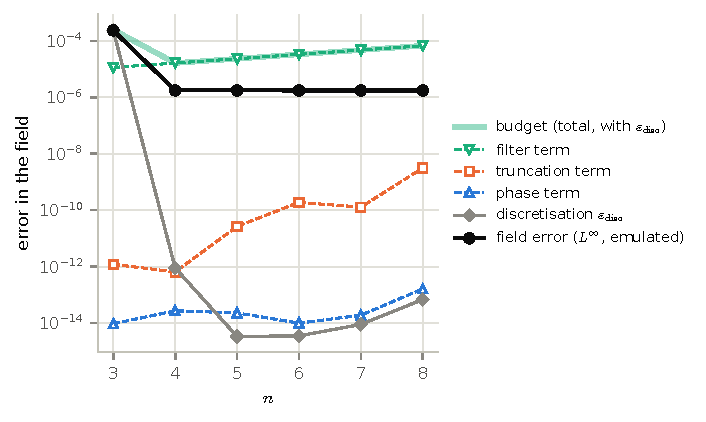
\includegraphics[width=0.72\linewidth]{Figs/decoded_field.pdf}
    \caption[Field error of the prepared state against its budget]{\textbf{From $n=4$ the filter, not the resolution, sets the prepared field's error, and the error budget bounds it with a margin that widens with $n$.} Against $n$ for R2a in the descriptor: the $L^\infty$ error of the field decoded classically from the prepared state, the discretisation's error $\varepsilon_{\mathrm{disc}}$, and the budget of \Cref{eq:error-budget}, whole (with $\varepsilon_{\mathrm{disc}}$) and as its filter, truncation and phase terms, each carried to the field by the readout bound (\Cref{prop:readout-bound}); minimax filter, $\varepsilon=10^{-6}$. The error follows $\varepsilon_{\mathrm{disc}}$ to $n=3$; from $n=4$ it holds at $\res[2,sci]{stateprep/R2a/descriptor/n8/T2/filter=minimax}{field_err_linf}$, because the filter leaves the same infidelity at every $n$, while $\varepsilon_{\mathrm{disc}}$ falls to rounding. The filter term, which carries that infidelity through the bound's worst direction, lies above the error and grows with $n$ as the bound's amplification $K$ does, from $\res[3]{stateprep/R2a/descriptor/n4/T2/filter=minimax}{kappa_read}$ at $n=4$ to $\res[3]{stateprep/R2a/descriptor/n8/T2/filter=minimax}{kappa_read}$ at $n=8$; the truncation and phase terms are negligible. Exact emulation.}
    \label{fig:decoded-field}
\end{figure}
